% !TeX spellcheck = en_US
%\documentclass[11pt,a4paper]{article}
\documentclass[11pt
  , a4paper
  , article
  , oneside
%  , twoside
%  , draft
]{memoir}

\usepackage{control}
\usepackage{kotex}
\usepackage[numbers]{natbib}
%\usepackage[pdftex]{graphicx}
%\DeclareGraphicsExtensions{.pdf,.png,.jpg}
\begin{document}

\newcommand{\technumber}{
  Digital Signal Processing using MATLAB\\
  Document 1: 2016-03-26}
\title{\textbf{Digital Signal Processing: 실습 6 \\
		제3장 이산시간 푸리에  변환의 성질 \\}}

\author{이상일\thanks{silee7103@ibs.re.kr} \\

  학번: 201460437\\
  Computer Engineering, Chungnam National University 
}
\date{\today}

\renewcommand{\maketitlehooka}{\begin{flushright}\textsf{\technumber}\end{flushright}}
%\renewcommand{\maketitlehookb}{\centering\textsf{\subtitle}}
%\renewcommand{\maketitlehookc}{C}
%\renewcommand{\maketitlehookd}{D}

\maketitle

\begin{abstract}
MATLAB을 사용한 Digital Signal Processing에 대한 실습과제에 대한 Documents를 구성한다.
\end{abstract}

\chapter{Example 3-18:}

\begin{lstlisting}[style=termstyle]
% Example 3.18
dt = 0.00005; t = -0.005:dt:0.005; xa = exp(-1000*abs(t));
Wmax = 2*pi*2000; K = 500; k = 0:1:K;
W = k*Wmax/K;
Xa = xa * exp(-j*t'*W) * dt; Xa = real(Xa);
W = [-fliplr(W), W(2:501)];
Xa = [fliplr(Xa), Xa(2:501)];
subplot(2,1,1);plot(t*1000,xa);
xlabel('t in msec.'); ylabel('xa(t)')
title('Analog Signal')

subplot(2,1,2);plot(W/(2*pi*1000),Xa*1000);
xlabel('Frequency in KHz'); ylabel('Xa(jW)*1000')
title('Continuous-time Fourier Transform')
\end{lstlisting}

\begin{figure}[h!]
	\centering
	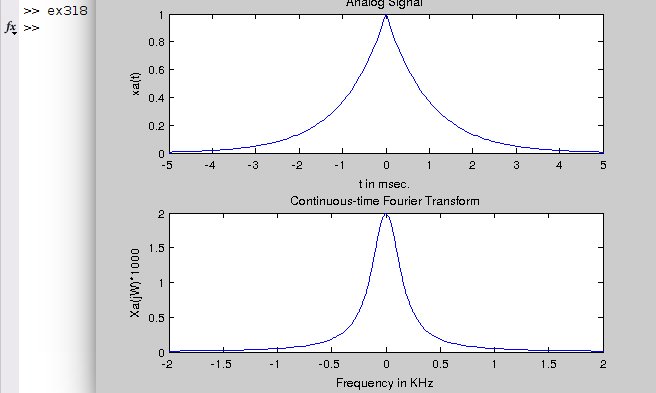
\includegraphics[width=0.7\textwidth,height=0.4\textwidth]{./images/ex318.png}
	\caption{Example 3.18 Result}
	\label{fig:Example 3-18 Result}
\end{figure}

\chapter{Example 3-19a:}

\begin{lstlisting}[style=termstyle]
% Example 3.19a
dt = 0.00005; t = -0.005:dt:0.005; 
xa = exp(-1000*abs(t));

Ts = 0.0002; n = -25:1:25; x = exp(-1000*abs(n*Ts));
K = 500; k = 0:1:K;
w = pi*k/K;

X = x * exp(-j*n'*w);
X = real(X);
w = [-fliplr(w), w(2:K+1)];
X = [fliplr(X), X(2:K+1)];

subplot(2,1,1);plot(t*1000,xa);
xlabel('t in msec.'); ylabel('x1(n)')
title('Discrete Signal'); hold on

stem(n*Ts*1000,x); gtext('Ts=0.2 msec'); hold off

subplot(2,1,2);plot(w/pi,X);
xlabel('Frequency in pi units'); ylabel('X1(w)')
title('Discrete-time Fourier Transform')
\end{lstlisting}

\clearpage

\begin{figure}[h!]
	\centering
	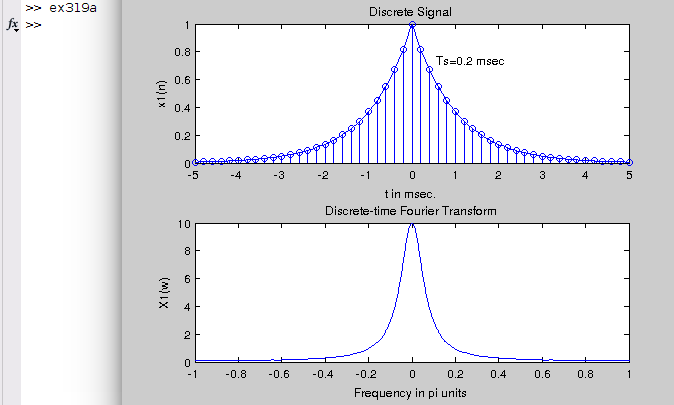
\includegraphics[width=0.7\textwidth,height=0.5\textwidth]{./images/ex319a.png}
	\caption{Example 3.19a Result}
	\label{fig:Example 3-19a Result}
\end{figure}

\clearpage

\chapter{Example 3-19b:}
\begin{lstlisting}[style=termstyle]
% Example 3.19b
dt = 0.00005; t = -0.005:dt:0.005; xa = exp(-1000*abs(t));
Ts = 0.001; n = -5:1:5;
x = exp(-1000*abs(n*Ts));
K = 500; k = 0:1:K;
w = pi*k/K;
X = x * exp(-j*n'*w);
X = real(X);
w = [-fliplr(w), w(2:K+1)];
X = [fliplr(X), X(2:K+1)];

subplot(2,1,1);plot(t*1000,xa);
xlabel('t in msec.'); ylabel('x2(n)')
title('Discrete Signal'); hold on

stem(n*Ts*1000,x); gtext('Ts=1 msec'); hold off

subplot(2,1,2);plot(w/pi,X);
xlabel('Frequency in pi units'); ylabel('X2(w)')
title('Discrete-time Fourier Transform')
\end{lstlisting}

\begin{figure}[h!]
	\centering
	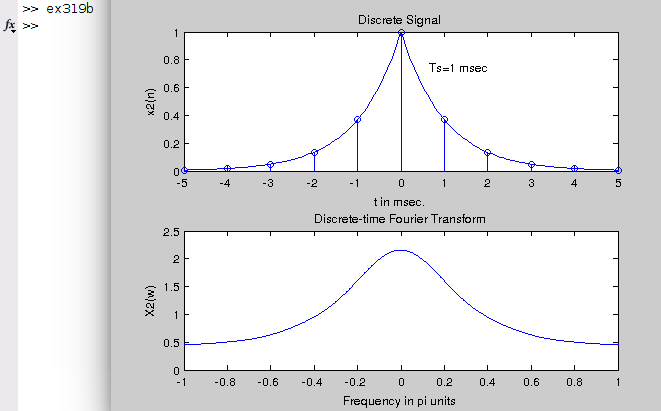
\includegraphics[width=0.7\textwidth,height=0.35\textwidth]{./images/ex319b.png}
	\caption{Example 3.19b Result}
	\label{fig:Example 3-19b Result}
\end{figure}

\chapter{Example 3-21:}
\begin{lstlisting}[style=termstyle]
% Example 3.21
ts = 0.0002; Fs = 1/ts; n = -25:1:25; nTs = n*ts;
x = exp(-1000*abs(nTs));
dt = 0.00005;
t = -0.005:dt:0.005;

xa = x * sinc(Fs*(ones(length(nTs),1)*t-nTs'*ones(1,length(t))));
error = max(abs(xa - exp(-1000*abs(t))))

subplot(2,1,2);plot(t*1000,xa);
xlabel('t in msec.'); ylabel('xa(t)')
title('Reconstructed Signal from x1(n) using sinc function'); hold on
stem(n*ts*1000,x); hold off
\end{lstlisting}

\clearpage

\begin{figure}[h!]
	\centering
	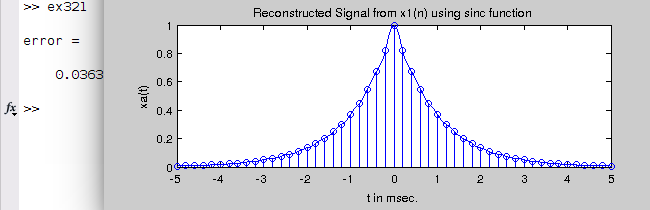
\includegraphics{./images/ex321.png}
	\caption{Example 3.21 Result}
	\label{fig:Example 3-21 Result}
\end{figure}

\chapter{Example 3-22:}
\begin{lstlisting}[style=termstyle]
% Example 3.22
ts = 0.001; Fs = 1/ts; n = -5:1:5; nTs = n*ts;
x = exp(-1000*abs(nTs));
dt = 0.00005;
t = -0.005:dt:0.005;

xa = x * sinc(Fs*(ones(length(nTs),1)*t-nTs'*ones(1,length(t))));
error = max(abs(xa - exp(-1000*abs(t))))

subplot(2,1,2);plot(t*1000,xa);
xlabel('t in msec.'); ylabel('xa(t)')
title('Reconstructed Signal from x2(n) using sinc function'); hold on
stem(n*ts*1000,x); hold off  
\end{lstlisting}

\begin{figure}[h!]
	\centering
	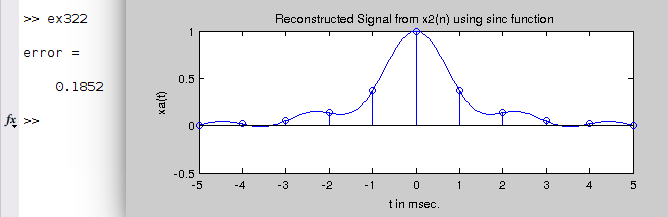
\includegraphics[width=0.7\textwidth,height=0.4\textwidth]{./images/ex322.png}
	\caption{Example 3.22 Result}
	\label{fig:Example 3-22 Result}
\end{figure}

\chapter{Example 3-23:}
\begin{lstlisting}[style=termstyle]
% Example 3.23
ts = 0.0002; n = -25:1:25; nTs = n*ts;
x = exp(-1000*abs(nTs));

subplot(2,1,1); stairs(nTs*1000,x);
xlabel('t in msec.'); ylabel('xa(t)')
title('Reconstructed Signal from x1(n) using zero-order-hold'); hold on
stem(n*ts*1000,x); hold off

subplot(2,1,2); plot(nTs*1000,x);
xlabel('t in msec.'); ylabel('xa(t)')
title('Reconstructed Signal from x1(n) using first-order-hold'); hold on
stem(n*ts*1000,x); hold off
\end{lstlisting}

\begin{figure}[h!]
	\centering
	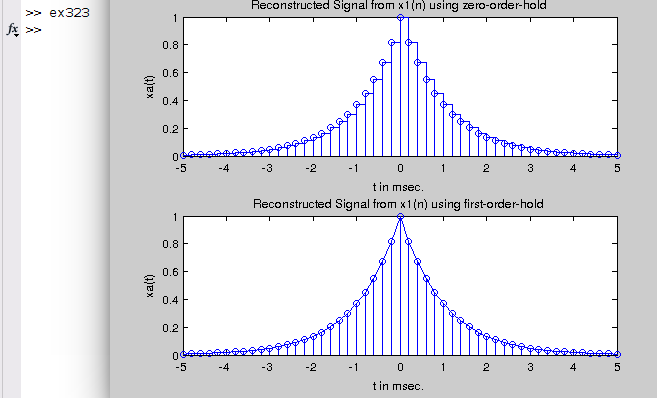
\includegraphics[width=0.7\textwidth,height=0.4\textwidth]{./images/ex323.png}
	\caption{Example 3.22 Result}
	\label{fig:Example 3-23 Result}
\end{figure}

\clearpage

\chapter{Problem 3-17:}
\section{1번: }
\begin{lstlisting}[style=termstyle]
%Problem 3.17-1
T_s1 = 0.01; n1 = [0:100]; x1 = cos(20*pi*n1*T_s1);
subplot(3,1,1); Hs = stem(n1,x1,'filled'); axis([-5 105 -1.2 1.2]);
set(Hs,'markersize',2); xlabel('n');
title(['x(n) = cos(20{\pi}nT_s) for T_s = 0.01 sec']);
ylabel('x(n)');
T_s2 = 0.05; n2 = [0:20]; x2 = cos(20*pi*n2*T_s2);
subplot(3,1,2); Hs = stem(n2,x2,'filled'); set(Hs,'markersize',2);
set(gca,'XTick',[0:20]); axis([-2 22 -1.2 1.2]);
xlabel('n');
ylabel('x(n)');
title(['x(n) = cos(20{\pi}nT_s) for T_s = 0.05 sec']);
T_s3 = 0.1; n3 = [0:10]; x3 = cos(20*pi*n3*T_s3);
subplot(3,1,3); Hs = stem(n3,x3,'filled'); set(Hs,'markersize',2);
set(gca,'XTick',[0:10]); axis([-1 11 -1.2 1.2]);
xlabel('n'); ylabel('x(n)');
title(['x(n) = cos(20{\pi}nT_s) for T_s = 0.1 sec']);
\end{lstlisting}

\begin{figure}[h!]
	\centering
	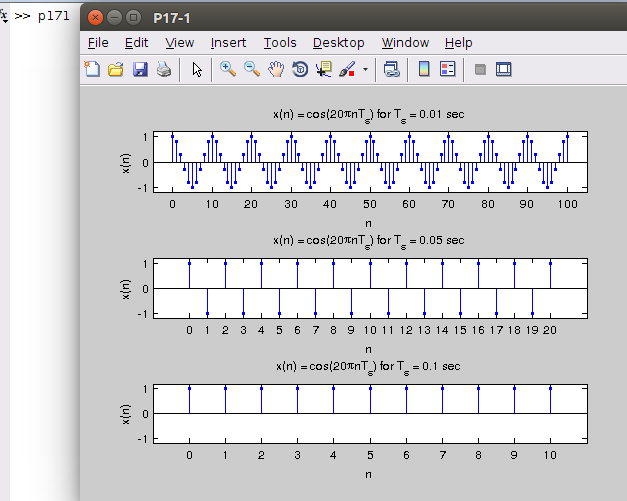
\includegraphics[width=0.7\textwidth,height=0.4\textwidth]{./images/p17-1.png}
	\caption{Problem 17-1 Result}
	\label{fig:Problem 17-1 Result}
\end{figure}

\section{2번: }
\begin{lstlisting}[style=termstyle]
%Problem 3.17-2
T_s1 = 0.01; n1 = [0:100]; x1 = cos(20*pi*n1*T_s1);
subplot(3,1,1); Hs = stem(n1,x1,'filled'); axis([-5 105 -1.2 1.2]);
set(Hs,'markersize',2); xlabel('n');
title(['x(n) = cos(20{\pi}nT_s) for T_s = 0.01 sec']);
ylabel('x(n)');
T_s2 = 0.05; n2 = [0:20]; x2 = cos(20*pi*n2*T_s2);
subplot(3,1,2); Hs = stem(n2,x2,'filled'); set(Hs,'markersize',2);
set(gca,'XTick',[0:20]); axis([-2 22 -1.2 1.2]);
xlabel('n'); ylabel('x(n)');
title(['x(n) = cos(20{\pi}nT_s) for T_s = 0.05 sec']);
T_s3 = 0.1; n3 = [0:10]; x3 = cos(20*pi*n3*T_s3);
subplot(3,1,3); Hs = stem(n3,x3,'filled'); set(Hs,'markersize',2)
set(gca,'XTick',[0:10]); axis([-1 11 -1.2 1.2]);
xlabel('n'); ylabel('x(n)');
title(['x(n) = cos(20{\pi}nT_s) for T_s = 0.1 sec']);
\end{lstlisting}

\begin{figure}[h!]
	\centering
	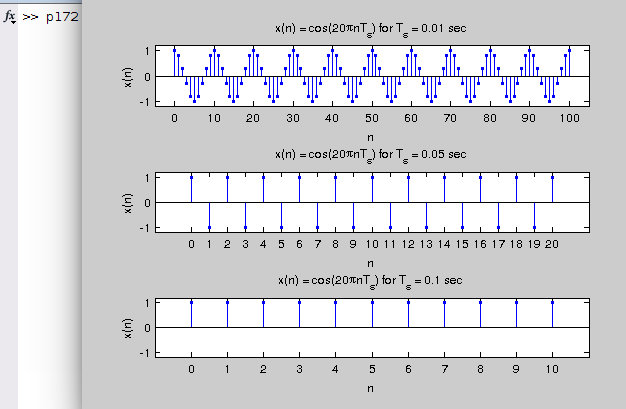
\includegraphics[width=0.7\textwidth,height=0.4\textwidth]{./images/p17-2.png}
	\caption{Problem 17-2 Result}
	\label{fig:Problem 17-2 Result}
\end{figure}

\section{3번: }
\begin{lstlisting}[style=termstyle]
%Problem 3.17-3
Ts1 = 0.01; Fs1 = 1/Ts1; n1 = [0:100]; nTs1 = n1*Ts1;
x1 = cos(20*pi*nTs1); Dt = 0.001; t = 0:Dt:1; xa1 = spline(nTs1,x1,t);
subplot(3,1,1); plot(t,xa1,'LineWidth',1.5); axis([0 1 -1.2 1.2]);
xlabel('t in sec'); ylabel('y_a(t)');
title(['Spline Interpolation: T_s = 0.01 sec']);
%
Ts2 = 0.05; Fs2 = 1/Ts2; n2 = [0:20]; nTs2 = n2*Ts2;
x2 = cos(20*pi*nTs2); Dt = 0.001; t = 0:Dt:1; xa2 = spline(nTs2,x2,t);
subplot(3,1,2); plot(t,xa2,'LineWidth',1.5); axis([0 1 -1.2 1.2]);
xlabel('t in sec'); ylabel('y_a(t)');
title(['Spline Interpolation: T_s = 0.05 sec']); grid;

Ts3 = 0.1; Fs3 = 1/Ts3; n3 = [0:10]; nTs3 = n3*Ts3; x3 = cos(20*pi*nTs3);
Dt = 0.001; t = 0:Dt:1; xa3 = spline(nTs3,x3,t);
subplot(3,1,3); plot(t,xa3,'LineWidth',1.5); axis([0 1 -1.2 1.2]);
xlabel('t in sec'); ylabel('y_a(t)');
title(['Spline Interpolation: T_s = 0.1 sec']); grid;
\end{lstlisting}

\begin{figure}[h!]
	\centering
	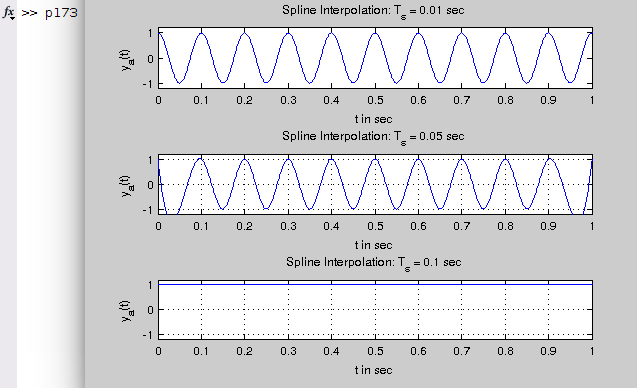
\includegraphics[width=0.7\textwidth,height=0.4\textwidth]{./images/p17-3.png}
	\caption{Problem 17-3 Result}
	\label{fig:Problem 17-3 Result}
\end{figure}

\clearpage

\section{4번: }
From the plots in Figures it is clear that reconstructions from samples at Ts = 0.01 and 0.05 depict the original frequency (excluding end effects) but reconstructions for Ts = 0.1 show the original frequency aliased to zero. Furthermore, the cubic spline interpolation is a better reconstruction than the sinc interpolation, that is, the sinc interpolation is more susceptible to boundary effect.


\chapter{Problem 3-18:}
\section{1번: }
\begin{lstlisting}[style=termstyle]
%Problem 3.18-1
Ts = 0.05; Fs = 1/Ts; Dt = 0.001; t = 0:Dt:1; n = [0:20]; nTs = n*Ts;
theta1 = 0; x_a1 = cos(20*pi*t+theta1); x1 = cos(20*pi*nTs+theta1);
subplot(5,1,1); plot(t,x_a1,'LineWidth',1.5); axis([0 1 -1.2 1.2]); hold on;
plot(nTs,x1,'o'); xlabel('t in sec');
title('x_a(t) and x(n) for \theta = 0');
ylabel('Amplitude');

theta2 = pi/6; x_a2 = cos(20*pi*t+theta2); x2 = cos(20*pi*nTs+theta2);
subplot(5,1,2); plot(t,x_a2,'LineWidth',1.5); axis([0 1 -1.2 1.2]); hold on;
plot(nTs,x2,'o'); xlabel('t in sec');
title('x_a(t) and x(n) for \theta = \pi/6');
ylabel('Amplitude');
theta3 = pi/4; x_a3 = cos(20*pi*t+theta3); x3 = cos(20*pi*nTs+theta3);
subplot(5,1,3); plot(t,x_a3,'LineWidth',1.5); axis([0 1 -1.2 1.2]); hold on;
plot(nTs,x3,'o'); xlabel('t in sec');
title('x_a(t) and x(n) for \theta = \pi/4');
ylabel('Amplitude');

theta4 = pi/3; x_a4 = cos(20*pi*t+theta4); x4 = cos(20*pi*nTs+theta4);
subplot(5,1,4); plot(t,x_a4,'LineWidth',1.5); axis([0 1 -1.2 1.2]); hold on;
plot(nTs,x4,'o'); xlabel('t in sec');
title('x_a(t) and x(n) for \theta = \pi/3');
ylabel('Amplitude');
theta5 = pi/2; x_a5 = cos(20*pi*t+theta5); x5 = cos(20*pi*nTs+theta5);
subplot(5,1,5); plot(t,x_a5,'LineWidth',1.5); axis([0 1 -1.2 1.2]); hold on;
plot(nTs,x5,'o'); xlabel('t in sec');
title('x_a(t) and x(n) for \theta = \pi/2');
ylabel('Amplitude');
\end{lstlisting}

\begin{figure}[h!]
	\centering
	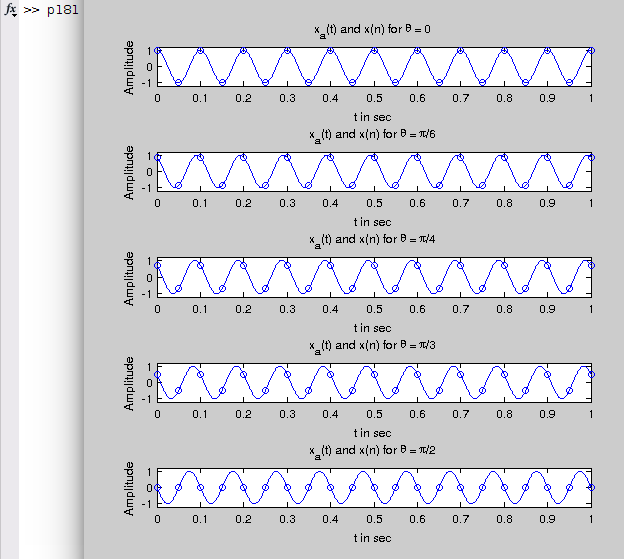
\includegraphics[width=0.7\textwidth,height=0.4\textwidth]{./images/p18-1.png}
	\caption{Problem 18-1 Result}
	\label{fig:Problem 18-1 Result}
\end{figure}

\clearpage

\section{2번: }
\begin{lstlisting}[style=termstyle]
%Problem 3.18-2
Ts = 0.05; Fs = 1/Ts; Dt = 0.001; t = 0:Dt:1; n = [0:20]; nTs = n*Ts;
theta1 = 0; x1 = cos(20*pi*nTs+theta1);
y_a1 = x1*sinc(Fs*(ones(length(n),1)*t-nTs'*ones(1,length(t))));
subplot(5,1,1); plot(t,y_a1,'LineWidth',1.5); hold on;
plot(nTs,x1,'o'); axis([0 1 -1.2 1.2]); xlabel('t in sec');
title('Sinc Interpolation for \theta = 0');
ylabel('Amplitude');
theta2 = pi/6; x2 = cos(20*pi*nTs+theta2);
y_a2 = x2*sinc(Fs*(ones(length(n),1)*t-nTs'*ones(1,length(t))));
subplot(5,1,2); plot(t,y_a2,'LineWidth',1.5); hold on; axis([0 1 -1.2 1.2])
plot(nTs,x2,'o'); xlabel('t in sec');
title('Sinc Interpolation for \theta = \pi/6');
ylabel('Amplitude');
theta3 = pi/4; x3 = cos(20*pi*nTs+theta3);
y_a3 = x3*sinc(Fs*(ones(length(n),1)*t-nTs'*ones(1,length(t))));
subplot(5,1,3); plot(t,y_a3,'LineWidth',1.5); hold on; axis([0 1 -1.2 1.2])
plot(nTs,x3,'o'); xlabel('t in sec');
title('Sinc Interpolation for \theta = \pi/4');
ylabel('Amplitude');
theta4 = pi/3; x4 = cos(20*pi*nTs+theta4);
y_a4 = x4*sinc(Fs*(ones(length(n),1)*t-nTs'*ones(1,length(t))));
subplot(5,1,4); plot(t,y_a4,'LineWidth',1.5); axis([0 1 -1.2 1.2]); hold on;
plot(nTs,x4,'o'); xlabel('t in sec');
title('Sinc Interpolation for \theta = \pi/3');
ylabel('Amplitude');
theta5 = pi/2; x5 = cos(20*pi*nTs+theta5);
y_a5 = x5*sinc(Fs*(ones(length(n),1)*t-nTs'*ones(1,length(t))));
subplot(5,1,5); plot(t,y_a5,'LineWidth',1.5); axis([0 1 -1.2 1.2]); hold on;
plot(nTs,x5,'o'); xlabel('t in sec');
title('Sinc Interpolation for \theta = \pi/3');
ylabel('Amplitude');
\end{lstlisting}

\begin{figure}[h!]
	\centering
	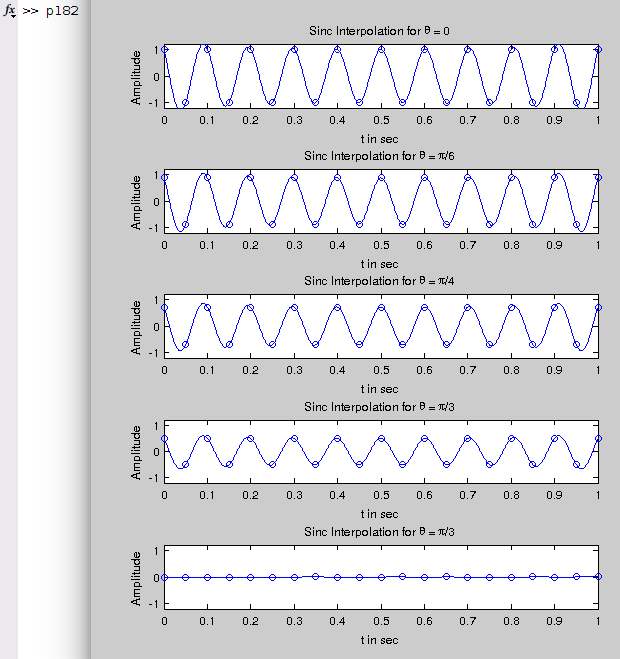
\includegraphics[width=0.7\textwidth,height=0.4\textwidth]{./images/p18-2.png}
	\caption{Problem 18-2 Result}
	\label{fig:Problem 18-2 Result}
\end{figure}

\clearpage

\section{3번: }
\begin{lstlisting}[style=termstyle]
%Problem 3.18-3
Ts = 0.05; Fs = 1/Ts; Dt = 0.001; t = 0:Dt:1; n = [0:20]; nTs = n*Ts;
theta1 = 0; x1 = cos(20*pi*nTs+theta1); y_a1 = spline(nTs,x1,t);
subplot(5,1,1); plot(t,y_a1,'LineWidth',1.5); axis([0 1 -1.2 1.2]); hold on;
plot(nTs,x1,'o'); xlabel('t in sec');
title('Spline Interpolation for theta = 0');
ylabel('Amplitude');
theta2 = pi/6; x2 = cos(20*pi*nTs+theta2); y_a2 = spline(nTs,x2,t);
subplot(5,1,2); plot(t,y_a2,'LineWidth',1.5); hold on; axis([0 1 -1.2 1.2]);
plot(nTs,x2,'o'); xlabel('t in sec');
title('Spline Interpolation for theta = \pi/6');
ylabel('Amplitude');
theta3 = pi/4; x3 = cos(20*pi*nTs+theta3); y_a3 = spline(nTs,x3,t);
subplot(5,1,3); plot(t,y_a3,'LineWidth',1.5); hold on; axis([0 1 -1.2 1.2]);
plot(nTs,x3,'o'); xlabel('t in sec');
title('Spline Interpolation for theta = \pi/3');
ylabel('Amplitude');
theta4 = pi/3; x4 = cos(20*pi*nTs+theta4); y_a4 = spline(nTs,x4,t);
subplot(5,1,4); plot(t,y_a4,'LineWidth',1.5); axis([0 1 -1.2 1.2]); hold on;
plot(nTs,x4,'o'); ylabel('Amplitude');
title('Spline Interpolation for theta = \pi');
xlabel('t in sec');
theta5 = pi/2; x5 = cos(20*pi*nTs+theta5); y_a5 = spline(nTs,x5,t);
subplot(5,1,5); plot(t,y_a5,'LineWidth',1.5); axis([0 1 -1.2 1.2]); hold on;
plot(nTs,x5,'o'); ylabel('Amplitude');
title('Spline Interpolation for theta = \pi/2');
xlabel('t in sec');
\end{lstlisting}

\begin{figure}[h!]
	\centering
	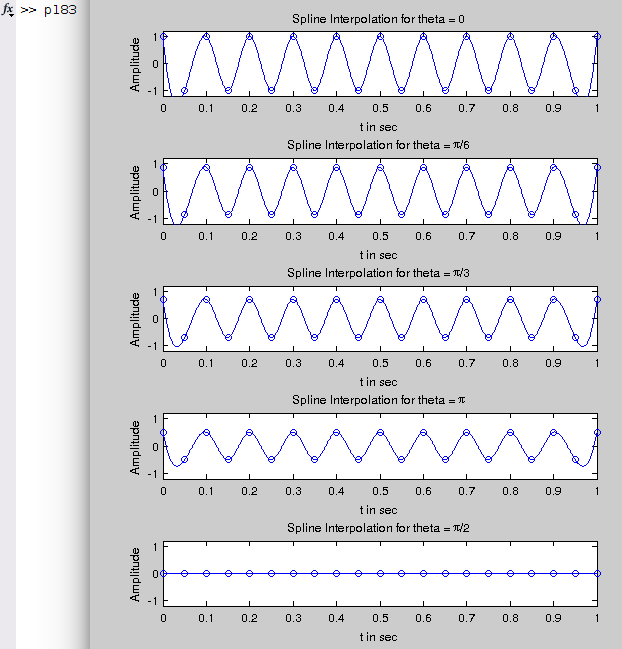
\includegraphics[width=0.7\textwidth,height=0.4\textwidth]{./images/p18-3.png}
	\caption{Problem 18-3 Result}
	\label{fig:Problem 18-3 Result}
\end{figure}

\section{4번: }
When a sinusoidal signal is sampled at f = 2 samples per cycle as is the case in this problem, then the resulting samples x(n) has the amplitude that depends on the phase of the signal. In particular note that this amplitude is given by cos(θ ). Thus the amplitude of the reconstructed signal y(t) is also equal to cos(θ ).


\end{document}

